\chapter{Planificación y análisis}
\label{cap:panificacion-analisis}

\section{Planificación}
\label{sec:planificacion}

Tras definir los objetivos a completar en el transcurso de este proyecto, pasamos a exponer la planificación temporal propuesta, que será dividida en diferentes fases y presentada, finalmente, mediante un diagrama de \textit{Gantt}.

\subsection{Fases}

A continuación se describen cada una de las fases propuestas así como una serie de actividades previstas por cada una de ellas.

\begin{itemize}
	\item \textbf{Fase 1}. Especificación del proyecto. Consiste en establecer los objetivos a cumplir para completar el proyecto, así como la búsqueda de información necesaria para llevarlo a cabo.
	\begin{itemize}
		\item Búsqueda de información.
		\item Determinación de objetivos.
		\item \underline{\textit{Estimación}}: 20 horas
	\end{itemize}
	
	\item \textbf{Fase 2}. Planificación. Elaboración y desarrollo de la documentación correspondiente a la planificación del proyecto.
	\begin{itemize}
		\item Listar las fases del proyecto.
		\item Especificar las actividades de las que constará cada fase.
		\item Temporización
		\item Análisis de presupuesto.
		\item \underline{\textit{Estimación}}: 20 horas
	\end{itemize}
	
	\item \textbf{Fase 3}. Análisis y diseño. Estudio del problema a abordar, análisis de requisitos y diagramas asociados de cara a concretar la forma en que se desarrollará.
	\begin{itemize}
		\item Análisis de requisitos
		\item Diseño de diagramas
		\item \underline{\textit{Estimación}}: 40 horas
	\end{itemize}
	
	\item \textbf{Fase 4}. Implementación. Tras las fases de planificación y diseño, se pasa a codificar todo lo necesario con el fin de cumplir los \hyperref[cap:objetivos]{objetivos propuestos}.
	\begin{itemize}
		\item Selección de herramientas.
		\item Desarrollo \textit{Backend}: modelos, \textit{urls}, controladores.
		\item Desarrollo \textit{Frontend}: vistas, \textit{templates}, \textit{HTML}, \textit{CSS}, \textit{Javascript}.
		\item Tareas de automatización (\textit{DevOps}).
		\item \underline{\textit{Estimación}}: 160 horas
	\end{itemize}
	
	\item \textbf{Fase 5}. Pruebas. Se hará uso de \textit{tests unitarios}, entre otros procedimientos, para probar el código generado y que el sistema funciona correctamente.
	\begin{itemize}
		\item Pruebas del software: modelos, vistas, formularios.
		\item \underline{\textit{Estimación}}: 35 horas
	\end{itemize}
	
	\item \textbf{Fase 6}. Documentación final. Completar la documentación restante asociada al proyecto, como manuales de usuario o anexos.
	\begin{itemize}
		\item Documentación del sistema.
		\item Manual de usuario.
		\item Documentación del proyecto.
		\item \underline{\textit{Estimación}}: 25 horas
	\end{itemize}
\end{itemize}

\subsection{Recursos humanos}

Además del autor del proyecto, se contempla la participación de representantes del público objetivo destinatario del producto con el fin de recabar información relativa a su utilidad, así como posibles deficiencias, beneficios y/o mejoras.


\subsection{Temporización}

Por último, para poder apreciar de una forma algo más visual la planificación temporal descrita, generamos un diagrama de \textit{Gantt} que represente dicha información.

\begin{figure}[H] 
\centering 
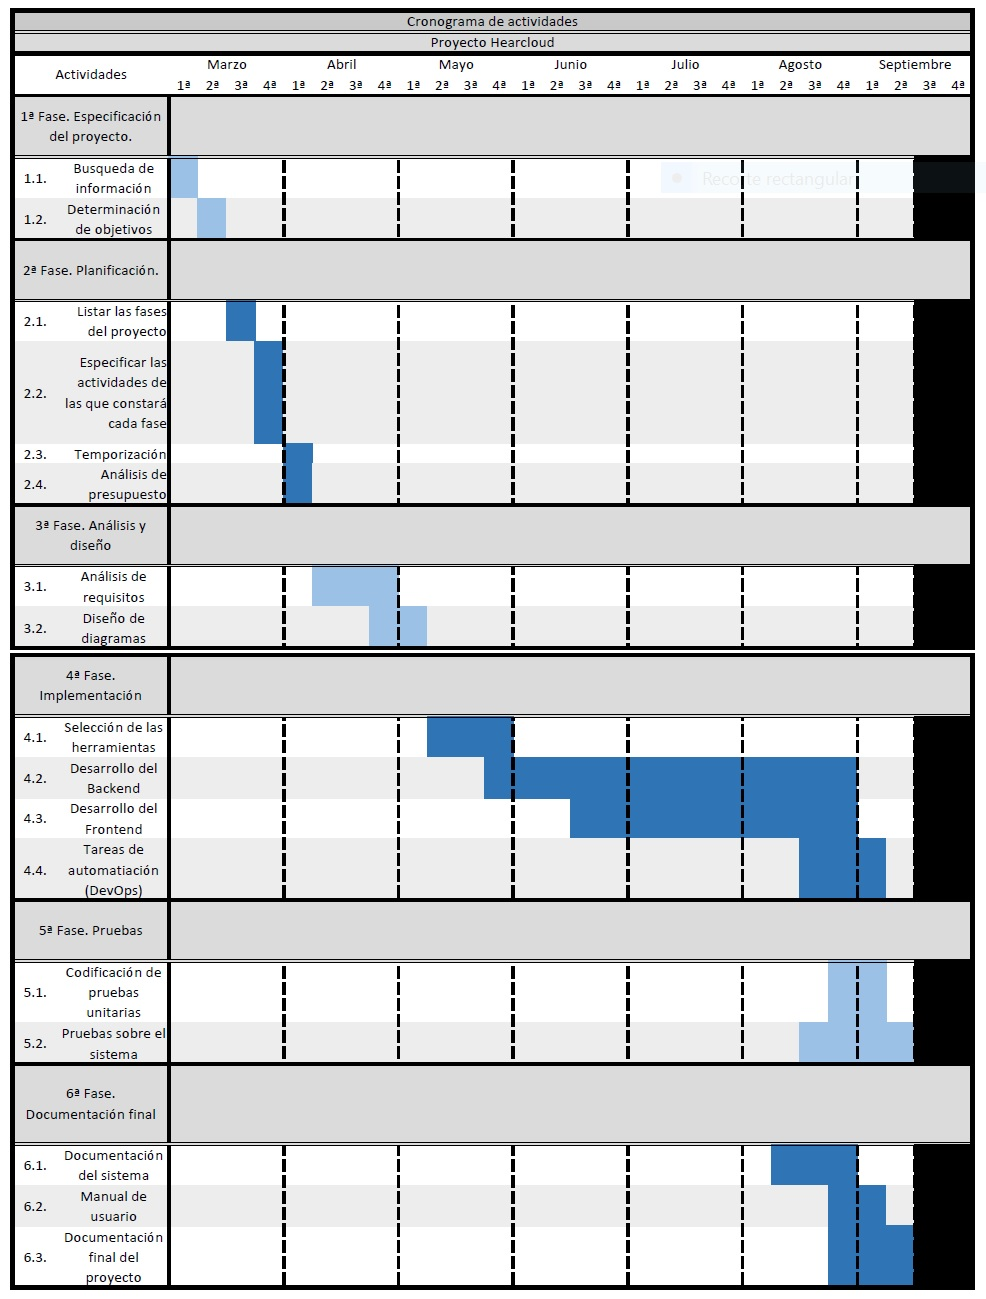
\includegraphics[scale=0.8]{../images/d_gantt.jpg}
\caption{Diagrama de Gantt del proyecto}
\end{figure}

\subsection{Presupuesto}

La principal ventaja del uso de software libre es que no es necesario adquirir licencias de pago para usar dicho software. Como las herramientas que se van a utilizar y todo el código que se genere será libre, el coste económico y, por tanto, el presupuesto inicial del proyecto será cero.\\

El único aspecto económico relevante que habrá que considerar en este caso será, entonces, el de los posibles gastos por el uso de un servidor en el que se implante el software.

\section{Análisis}
\label{sec:analisis}

\subsection{Estudio de mercado}

La creación de un producto software nuevo no es una tarea sencilla, sobre todo cuando no cuentas con una mínima información acerca del mercado en el que esperas que se desenvuelva. Por eso, realizar un estudio de las alternativas ya existentes, nos ayudará a obtener datos sobre nuestros ``competidores'' y localizar posibles enfoques promocionales de cara a resaltar las ventajas que nuestra solución pueda ofrecer frente a las suyas. Entre ellos, destacamos:

\subsubsection{Spotify \cite{Spotify}}
Spotify es un servicio de reproducción de música vía streaming que permite escuchar un amplio catálogo en modo radio o bien buscando por artista, álbum o listas de reproducción. Si embargo, éste es ofrecido por la plataforma y no es posible almacenar tu própia música en ella para combinarlo, de alguna manera, con lo que ya ofrecen ellos. Por tanto, si una canción no se encuentra entre sus bases de datos, tendrás que recurrir a otra alternativa para poder oirla. No obstante, si no es el caso, la plataforma representa una gran ventaja para disponer de tu selección musical en la nube y organizada según tus propios criterios en modo de listas de reproducción.\\

El servicio puede utilizarse de dos formas diferentes: la versión gratuita, con la publicidad ocasional mencionada y la limitación de no poder escuchar canciones bajo demanda en la versión móvil, y la versión ``\textit{premium}'', que elimina todas estas limitaciones, ofrece una calidad de audio mejor y la posibilidad de descargar la música para escucharla en modo sin conexión.

\subsubsection{Soundcloud \cite{Soundcloud}}
Soundcloud es una plataforma de distribución de audio en línea que permite a sus usuarios subir, grabar, promocionar y compartir su música de autoría original. Está, por tanto, orientada sobre todo a músicos y sellos discográficos, aunque cualquier usuario registrado tiene acceso a la música de estos y puede almacenarla en listas de reproducción, públicas o privadas, en su propio perfil para su reproducción.\\

La plataforma ofrece servicios premium en dos modalidades diferentes: ``\textit{Pro}'', que permite subir hasta seis horas de audio y, estadísticas ampliadas sobre los usuarios que reproducen tu música o deshabilitar comentarios y ``\textit{Pro Unlimited}'', que permite subir horas ilimitadas de música al usuario.

\subsubsection{Amazon Cloud Player \cite{ACP}} 
Amazon Cloud Player es un servicio integrado con la plataforma Amazon Music que permite al usuario almacenar y reproducir su música desde el navegador, aplicaciones móviles y de escritorio, Sonos y otras plataformas como televisiones inteligentes (se permiten hasta 10 dispositivos, que pueden autorizarse y desautorizarse desde la interfaz web). La capacidad de almacenamiento está limitada a 5GB y 250 canciones de forma gratuita, sin contar la música comprada a través de Amazon Music. Con la suscripción a Amazon Music, se puede ampliar el número hasta 250.000. Además, se permiten editar algunos metadatos de dichos ficheros, como el título, artista o álbum. La única limitación del servicio es que, aún para usar la cuenta gratuita, es necesario introducir un número de tarjeta de crédito en el sistema.

\subsubsection{Google Play Music \cite{GPM}}
Google Play Music es un servicio de almacenamiento y sincronización de música en la nube, a la vez que tienda musical en línea que forma parte de Google Play. Éste permite el almacenamiento gratuito de canciones propias hasta un total de 50.000 que, al sincronizarse en la nube, están disponibles desde cualquier punto. La suscripción ''\textit{all access}'' permite la reproducción en streaming bajo demanda de cualquier canción del catálogo de la tienda. Con la aplicación móvil, podremos almacenar la música de forma local para poder escucharla en modo \textit{offline}. No obstante, los usuarios deberán verificar su ubicación aportando un número de tarjeta de crédito válido a su cuenta de Google antes de poder ingresar por primera vez a la plataforma.\\

Durante el proceso de subida, el sistema intentará encontrar alguna coincidencia con el catálogo de Google Play y, si se encuenta alguno, la canción se añadirá a la librería del usuario sin la necesidad de que esta se termine de subir. Además, el servicio permite la creación de listas de reproducción automática, característica conocida como ``\textit{Instant Mix}, y recibir recomendaciones personalizadas teniendo en cuenta lo que más reproduzcas.

\subsubsection{My Music Cloud \cite{MMC}}
My Music Cloud es una plataforma que permite almacenar la música de sus usuarios en todos sus dispositivos y que dispone de un reproductor personalizado e inteligente. La aplicación sincroniza la música del usuario desde cualquier ordenador, \textit{smart phone}, tablet o televisión y, una vez subida, puede reproducirla, incluso sin conexión. La versión gratuita permite subir cuanta música se quiera, aunque solamente podrán sincronizarse con los diferentes dispositivos 250. Al igual que los servicios anteriores, también dispone de una tienda online, aunque mucho más limitada en cuanto a catálogo ofertado. No obstante, los ficheros subidos por el usuario no están accesible para otros. Además, pueden editar los metadatos básicos de cada fichero. Los formatos soportados son: aac, mp3, ra, wav, wma, m4a, ogg, 3g2, 3gp, 3gpp and 3gpp2, flac, siempre y cuando cada fichero ocupe menos de 100MB. La opción de pago amplía el numero máximo de dispositivos a sincronizar de 5 a 10, permite sincronizar y reproducir pistas ilimitadamente y elimina los anuncios.

\subsection{Análisis de requisitos}

\subsubsection{Requisitos funcionales}
A continuación se expone una descripción de los requisitos más importantes a nivel de funciones que debe incluir el sistema, realizando una clasificación en categorías. A cada uno de los requisitos se le ha asignado un código y nombre con el fin de identificarlo fácilmente a lo largo de todo el proyecto.

\begin{itemize}
	\item \textbf{RF-1. Gestión de usuarios}. Mantener un control de los usuarios dados de alta en el sistema en cada momento y controlar su rol en él.
	\begin{itemize}
		\item \textbf{RF-1.1. Dar de alta a un usuario} si no posee ya cuenta y desea subir una canción o crear una lista de reproducción.
		\item \textbf{RF-1.2. Dar de baja a un usuario}. Si el usuario no desea seguir afiliado a la página debe poder darse de baja en cualquier momento, desapareciendo de ese modo toda su información de la página.
		\item \textbf{RF-1.3. Consulta de información}. Cualquier usuario puede ver la información relacionada con él, como su nombre de usuario, correo electrónico o imagen de perfil, así como sus canciones y listas de reproducción.
		\item \textbf{RF-1.4. Modificación de datos}. El usuario podrá modificar sus datos personales, nombre de usuario(siempre que esté disponible) y eliminar cualquiera de sus canciones y/o listas de reproducción.
	\end{itemize}				
	
	\item \textbf{RF-2. Gestión de canciones}. Se permite crear/eliminar cualquier canción de la base de datos, así como consultar/modificar cualquiera de sus datos.
	\begin{itemize}
		\item \textbf{RF-2.1. Añadir canciones}. Cada canción tiene asociados una serie de metadatos, los cuales se tomaran a partir del fichero subido al sistema.
		\item \textbf{RF-2.2. Eliminar canciones}. Se eliminará del sistema toda la información relativa a la canción, incluyendo su imagen y fichero asociados.
		\item \textbf{RF-2.3. Consultar canciones}. Se mostrarán los datos relativos a una canción.
		\item \textbf{RF-2.4. Modificar canción}. Se actualizarán los campos modificados de los metadatos de la canción, tanto en la base de datos como en el fichero asociado.
	\end{itemize}
	
	\item \textbf{RF-3. Gestión de listas de reproducción}. Se permite crear/eliminar listas de reproducción de la base de datos, así como consultar/modificar cualquiera de sus datos.
	\begin{itemize}
		\item \textbf{RF-3.1. Crear listas de reproducción}. Cada lista de reproducción puede contener una o más canciones. Si no contiene ninguna, la lista de reproducción estará vacía.
		\item \textbf{RF-3.2. Eliminar listas de reproducción}. Se eliminará del sistema la lista de reproducción indicada y las canciones que ésta pueda contener se desvincularán de ella.
		\item \textbf{RF-3.3. Consultar listas de reproducción}. Se mostrarán los datos relativos a la lista de reproducción, como su nombre o canciones que contiene.
		\item \textbf{RF-3.4. Modificar lista de reproducción}. Se actualizan los campos modificados de la lista de reproducción, incluidas las canciones que se seleccionen como contenidas en ella.
	\end{itemize}	 
\end{itemize}
\subsubsection{Requisitos no funcionales}
Aquí se incluyen algunas restricciones que afectarán a los requisitos anteriores.

\begin{itemize}

	\item \textbf{RNF-1. Seguridad de la información}. Ante un posible fallo del sistema, no debe perderse la información previamente almacenada. En un principio esto está garantizado, ya que sistema y base de datos serán entidades relacionadas pero no aisladas. No obstante, será buena práctica tener en cuenta la posibilidad de realizar copias de seguridad periódicamente o alguna otra alternativa que permita replicar los datos.

	\item \textbf{RNF-2. Concurrencia}. Tanto administradores como usuarios podrán trabajar simultáneamente con el sistema,
introduciendo información, consultándola o modificándola.

	\item \textbf{RNF-3. Autenticación}. Es necesario controlar las diferentes restricciones de los usuarios (administradores y usuarios comunes), de manera que cada uno pueda realizar sólo determinadas tareas.

	\item \textbf{RNF-4. Legales}. Deben tenerse en cuenta ciertos criterios de responsabilidad sobre los datos publicados, como que los datos de un usuario, no sean accesibles a otro. No obstante, y como puede consultarse en esta referencia \cite{GMELNEL}, el responsable último de los datos subidos a la plataforma, será el usuario.
	
	\item \textbf{RNF-5. Rendimiento}. El sistema debe tener un tiempo de respuesta y aprovechamiento de los recursos
óptimo.

\end{itemize}

\subsubsection{Requisitos de información}
A continuación se indica la información que es necesario almacenar en el sistema.

\begin{itemize}
	\item \textbf{RI-1. Usuarios}. Datos sobre las personas que integrarán el sistema que se va a desarrollar.
	\begin{itemize}
		\item \underline{Contenido}: nombre de usuario, clave de acceso, dirección de correo electrónico, nombre, apellidos, rol.
		\item \underline{Requisitos asociados}: RF-1, RNF-1, RNF-3.
	\end{itemize}
	
	\item \textbf{RI-2. Canciones}. Datos técnicos sobre las canciones almacenadas en el sistema.
	\begin{itemize}
		\item \underline{Contenido}: fichero, nombre del fichero original, tamaño del fichero, tipo de fichero, título, artista, álbum, fecha de publicación, artista del álbum, número de pista, número de pistas del álbum, \textit{Beats Per Minute} (BPM), artista original, tonalidad, compositor, compositor de la letra, comentarios, remezclador, sello discográfico, género, usuario al que pertenece, playlists en las que se encuentra incluida.
		\item \underline{Requisitos asociados}: RF-2, RF-3, RNF-1, RNF-3, RNF-4, RNF-5
	\end{itemize}
	
	\item \textbf{RI-3. Listas de reproducción}. Contendrá la información relacionada con las listas de reproducción creadas por los usuarios del sistema.
	\begin{itemize}
		\item \underline{Contenido}: título de la lista de reproducción, usuario que la creó y canciones incluidas en ella.
		\item \underline{Requisitos asociados}: RF-2, RF-3, RNF-1, RNF-3, RNF-4, RNF-5
	\end{itemize}
	
\end{itemize}

\subsubsection{Casos de uso}

\paragraph{Descripción de los actores}

\begin{itemize}
	\item \textbf{AC-1. Administrador}.
	\begin{itemize}
		\item \textbf{Descripción}. Gestiona la página web, desde dar de alta a usuarios, hasta modificar cualquier tipo de información relacionada con éstos, darlos de baja o controlar el acceso de otros administradores.
		\item \textbf{Características}. Conocimientos avanzados sobre creación y administración de páginas web.
		\item \textbf{Relaciones}. Se relaciona con los demás usuarios del sistema.
		\item \textbf{Referencias}. Interviene en la administración de usuarios, canciones y listas de reproducción.
		\item \textbf{Atributos}.
		\begin{itemize}
			\item \textbf{Nombre de usuario}: pseudónimo de acceso al sistema.
			\item \textbf{Correo electrónico}: correo electrónico de contacto.
			\item \textbf{Contraseña}. Clave de acceso al sistema.
			\item \textbf{Datos personales}: nombre y apellidos.
		\end{itemize}
	\end{itemize}
	
	\item \textbf{AC-2. Usuario}.
	\begin{itemize}
		\item \textbf{Descripción}. Usuario que accede al sistema para consultar su colección de canciones y listas de reproducción o crear y almacenar nuevas.
		\item \textbf{Características}. Interés por la música, conocimientos básicos sobre el manejo de ordenadores o dispositivos móviles para acceder y manejar el sistema.
		\item \textbf{Relaciones}. Sin relación con otros usuarios del sistema.
		\item \textbf{Referencias}. Puede consultar la base de datos de sus canciones, sus listas de reproducción y datos asociados con su perfil.
		\item \textbf{Atributos}.
		\begin{itemize}
			\item \textbf{Nombre de usuario}: pseudónimo de acceso al sistema.
			\item \textbf{Correo electrónico}: correo electrónico de contacto.
			\item \textbf{Contraseña}. Clave de acceso al sistema.
			\item \textbf{Datos personales}: nombre y apellidos.
		\end{itemize}
	\end{itemize}
\end{itemize}

\paragraph{Diagramas del modelo de casos de uso} \mbox{}\\

Los diagramas de casos de uso representan cómo los diferentes actores se relacionan con el sistema para usar sus funciones. A continuación se muestran los diagramas generados.

\begin{figure}[H]
  \begin{center}
  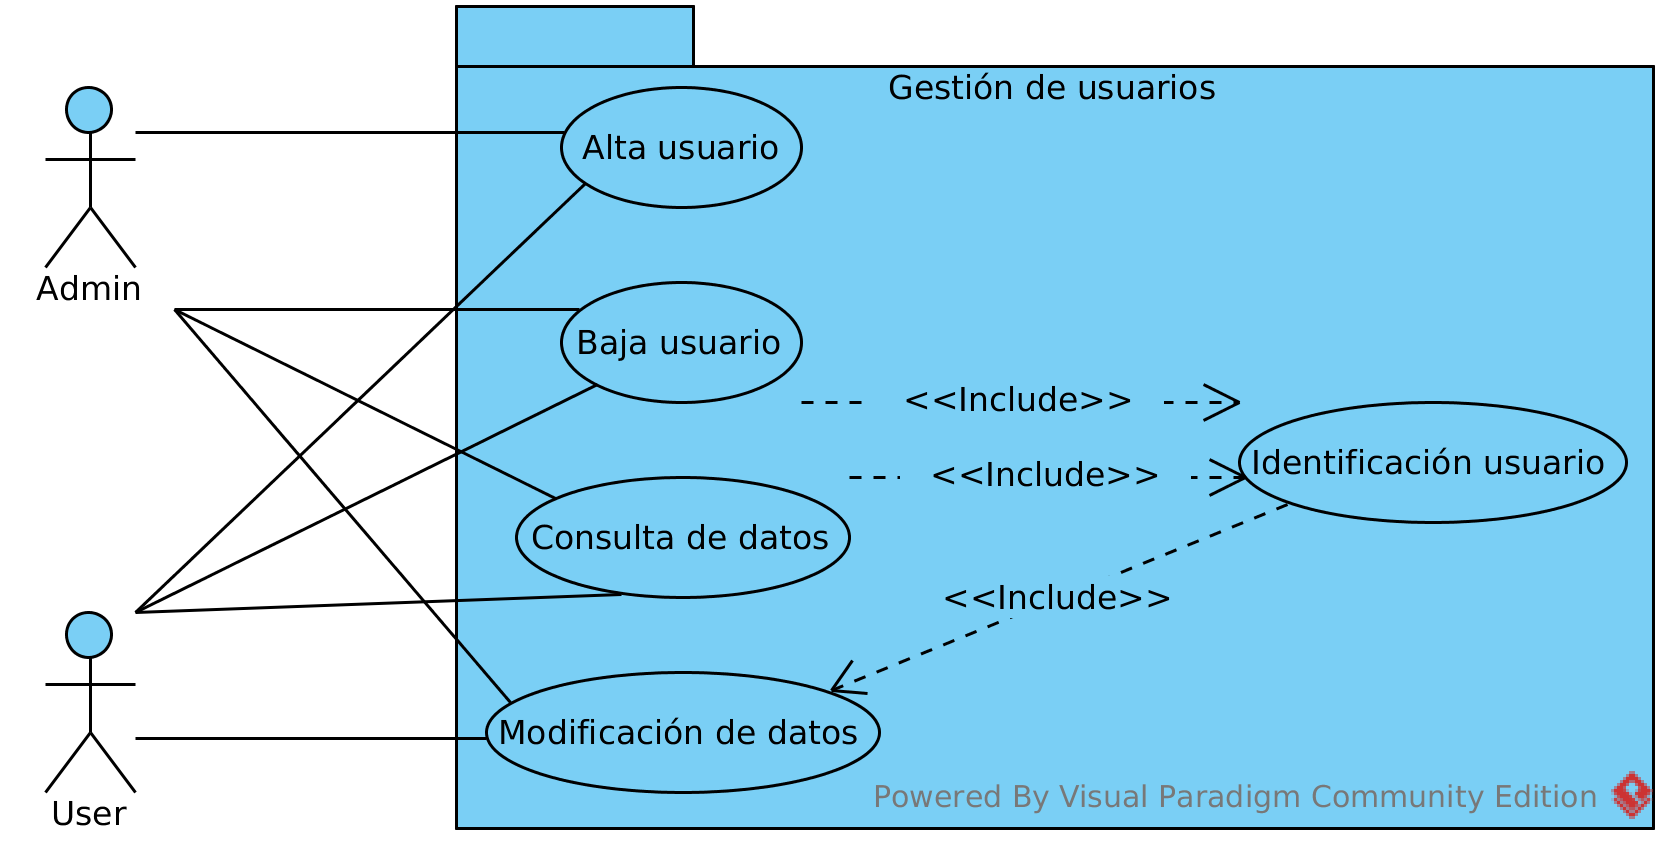
\includegraphics[width=0.65\textwidth]{../visual_paradigm_uml/CU-1_Gestion_de_usuarios.png}
  \caption{Diagrama de casos de uso. Gestión de usuarios}
  \label{fig:diag_cu_gu}
  \end{center}
\end{figure}

\begin{figure}[H]
  \begin{center}
  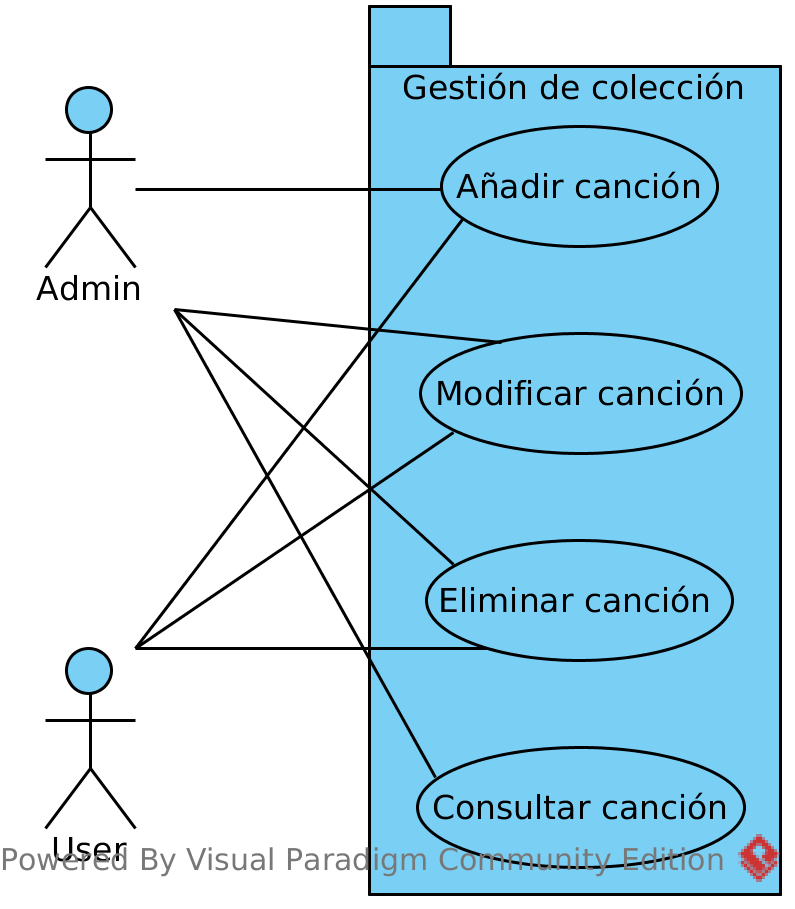
\includegraphics[width=0.4\textwidth]{../visual_paradigm_uml/CU-2_Gestion_de_canciones.png}
  \caption{Diagrama de casos de uso. Gestión de canciones}
  \label{fig:diag_cu_gc}
  \end{center}
\end{figure}

\begin{figure}[H]
  \begin{center}
  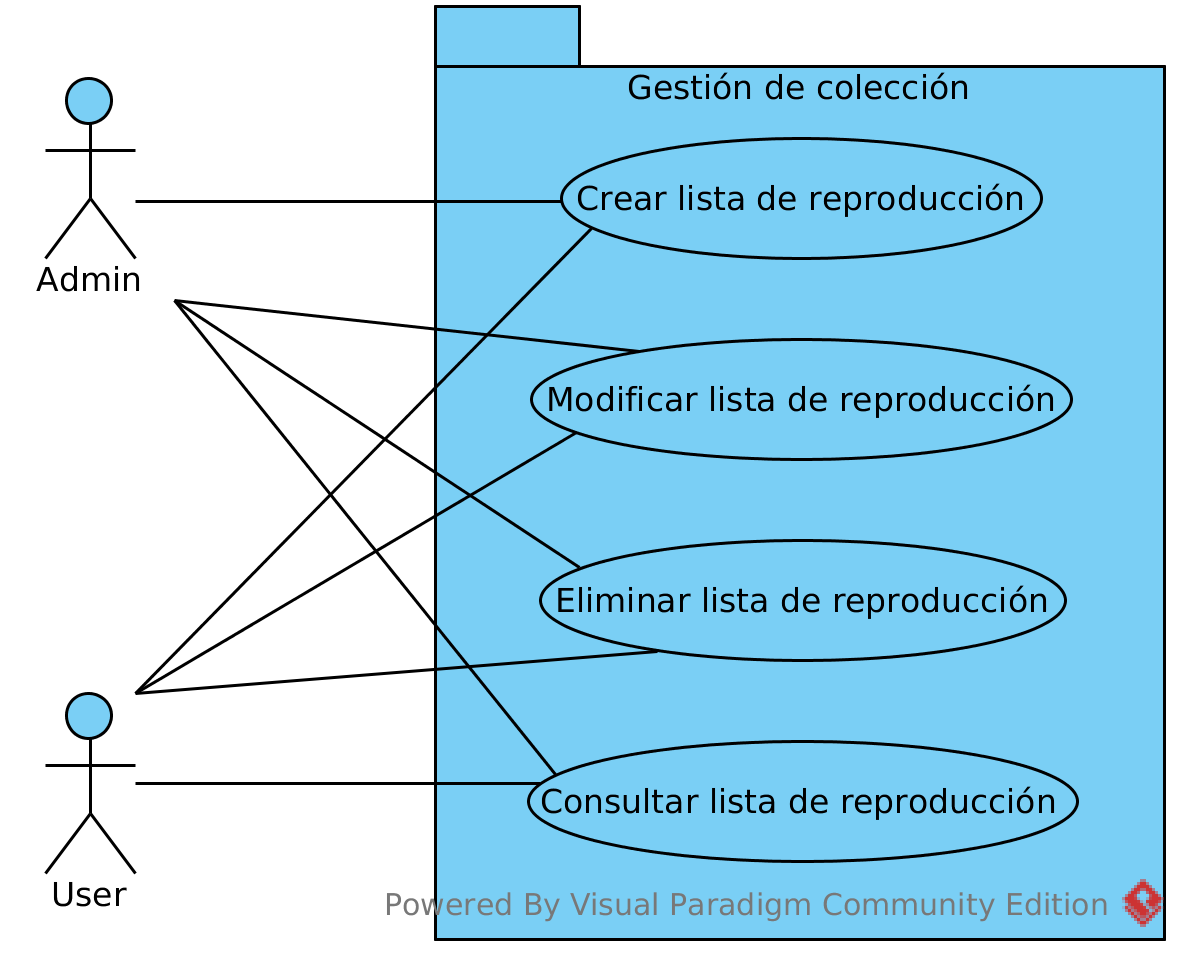
\includegraphics[width=0.65\textwidth]{../visual_paradigm_uml/CU-3_Gestion_de_listas_de_reproduccion.png}
  \caption{Diagrama de casos de uso. Gestión de listas de reproducción}
  \label{fig:diag_cu_glr}
  \end{center}
\end{figure}

\paragraph{Descripción de los casos de uso} \mbox{}

A continuación se exponen los casos de uso principales del sistema, correspondientes a las
acciones básicas del usuario con la plataforma, definiendo el comportamiento normal y
alternativo de cada acción.

% CASO DE USO 1
\textbf{CU-1.} Registro de usuarios (\textit{Sign Up}).
  
\begin{itemize}
    \item Descripción: el usuario se registrará con sus datos en el sistema.
    \item Precondición: el usuario no se encuentra registrado en el sistema.
    \item Postcondición: el usuario quedará registrado en el sistema con los datos proporcionados y se le asignará un identificador único.
\end{itemize}
    
\begin{table}[H]
  \begin{center}
    \begin{tabular}{|l|l|l|l|}
      \hline
      \multicolumn{4}{|c|}{{\bf Curso normal}}
      \\ \hline
      \multicolumn{2}{|c|}{{\bf Actor}} & \multicolumn{2}{|c|}{{\bf Sistema}}
      \\ \hline
      {\it 1} & 
      \begin{tabular}[c]{@{}l@{}}
        Usuario: inicia la acción\\
        de registro en el sistema.
      \end{tabular} &
      &
      \\ \hline
      &
      &
      {\it 2a} &
      \begin{tabular}[c]{@{}l@{}}
        Dar de alta al usuario en\\
        el sistema.
      \end{tabular}
      \\ \hline
      &
      &
      {\it 3} &
      \begin{tabular}[c]{@{}l@{}}
        El usuario queda dado de\\
        alta en el sistema y ya\\
        puede acceder.
      \end{tabular}
      \\ \hline
    \end{tabular}
    \caption{Curso normal de CU-1. Registro de usuarios.}
    \label{table:cn_cu_1}
  \end{center}
\end{table}

\begin{table}[H]
  \begin{center}
    \begin{tabular}{|l|l|}
      \hline
      \multicolumn{2}{|c|}{{\bf Curso alterno}}
      \\ \hline
      {\it 2b} &
      \begin{tabular}[c]{@{}l@{}}
        Si alguno de los datos que identifican al usuario se encuentran\\
        ya registrados en el sistema o alguno de ellos es inválido, no\\
        se continúa y se notifica el error al usuario.
      \end{tabular}\\
      \hline
    \end{tabular}
    \caption{Curso alterno de CU-1. Registro de usuarios.}
    \label{table:ca_cu_1}
  \end{center}
\end{table}

% CASO DE USO 2
\textbf{CU-2.} Identificación de usuarios (\textit{Log In}).

\begin{itemize}
    \item Descripción: el usuario iniciará con sus datos de acceso una sesión en el sistema.
    \item Precondición: el usuario se encuentra registrado en el sistema
    \item Postcondición: el usuario obtiene acceso al sistema y queda identificado en él, iniciándose su sesión.
\end{itemize}

\begin{table}[H]
  \begin{center}
    \begin{tabular}{|l|l|l|l|}
      \hline
      \multicolumn{4}{|c|}{{\bf Curso normal}}
      \\ \hline
      \multicolumn{2}{|c|}{{\bf Actor}} & \multicolumn{2}{|c|}{{\bf Sistema}}
      \\ \hline
      {\it 1} & 
      \begin{tabular}[c]{@{}l@{}}
        Usuario: inicia sesión.
      \end{tabular} &
      &
      \\ \hline
      &
      &
      {\it 2a} &
      \begin{tabular}[c]{@{}l@{}}
        Inicia la sesión del usuario\\
        en el sistema y genera un hash\\
        con el id de sesión que se enviará\\
        al usuario.
      \end{tabular}
      \\ \hline
      &
      &
      {\it 3} &
      \begin{tabular}[c]{@{}l@{}}
        El usuario queda logeado\\
        en el sistema y ya\\
        puede acceder.
      \end{tabular}
      \\ \hline
    \end{tabular}
    \caption{Curso normal de CU-2. Identificación de usuarios.}
    \label{table:cn_cu_2}
  \end{center}
\end{table}

\begin{table}[H]
  \begin{center}
    \begin{tabular}{|l|l|}
      \hline
      \multicolumn{2}{|c|}{{\bf Curso alterno}}
      \\ \hline
      {\it 2b} &
      \begin{tabular}[c]{@{}l@{}}
        Si alguno de los datos que identifican al usuario no coinciden\\
        con los almacenados en el sistema o alguno de ellos es inválido,\\
        no se continúa y se notifica el error al usuario.
      \end{tabular}\\
      \hline
    \end{tabular}
    \caption{Curso alterno de CU-2. Identificación de usuarios.}
    \label{table:ca_cu_2}
  \end{center}
\end{table}

% CASO DE USO 3
\textbf{CU-3.} Añadir canción.
  
\begin{itemize}
    \item Descripción: se añade una canción a la colección del usuario.
    \item Precondición: el usuario se encuentra con una sesión iniciada en el sistema
    \item Postcondición: se vincula la canción subida al usuario cuya sesión se encontraba iniciada en el momento de subirse a la plataforma.
\end{itemize}

\begin{table}[H]

  \begin{center}
    \begin{tabular}{|l|l|l|l|}
      \hline
      \multicolumn{4}{|c|}{{\bf Curso normal}}
      \\ \hline
      \multicolumn{2}{|c|}{{\bf Actor}} & \multicolumn{2}{|c|}{{\bf Sistema}}
      \\ \hline
      {\it 1} & 
      \begin{tabular}[c]{@{}l@{}}
        Usuario: selecciona un fichero\\
        de audio para subirlo a la\\
        plataforma.
      \end{tabular} &
      &
      \\ \hline
      &
      &
      {\it 2a} &
      \begin{tabular}[c]{@{}l@{}}
        El fichero se sube al sistema\\ 
        y se procesa.
      \end{tabular}
      \\ \hline
      &
      &
      {\it 3} &
      \begin{tabular}[c]{@{}l@{}}
        La canción queda vinculada\\
        con el usuario y se añade\\
        como parte de su colección.
      \end{tabular}
      \\ \hline
    \end{tabular}
    \caption{Curso normal de CU-3. Añadir canción.}
    \label{table:cn_cu_3}
  \end{center}
\end{table}

\begin{table}[H]
  \begin{center}
    \begin{tabular}{|l|l|}
      \hline
      \multicolumn{2}{|c|}{{\bf Curso alterno}}
      \\ \hline
      {\it 2b} &
      \begin{tabular}[c]{@{}l@{}}
        Si el formato del fichero no es válido o se cancela la subida por\\
        cualquier motivo, la canción no se añade al sistema y se notifica\\
        al usuario el error.
      \end{tabular}\\
      \hline
    \end{tabular}
    \caption{Curso alterno de CU-3. Añadir canción.}
    \label{table:ca_cu_3}
  \end{center}
\end{table}

% CASO DE USO 4
\textbf{CU-4.} Consultar canción.
  
\begin{itemize}
    \item Descripción: se muestran los datos solicitados de una canción.
    \item Precondición: el usuario se encuentra con una sesión iniciada en el sistema.
    \item Postcondición: el sistema devuelve los datos.
\end{itemize}

\begin{table}[H]

  \begin{center}
    \begin{tabular}{|l|l|l|l|}
      \hline
      \multicolumn{4}{|c|}{{\bf Curso normal}}
      \\ \hline
      \multicolumn{2}{|c|}{{\bf Actor}} & \multicolumn{2}{|c|}{{\bf Sistema}}
      \\ \hline
      {\it 1} & 
      \begin{tabular}[c]{@{}l@{}}
        Usuario: selecciona una canción para\\
        consultar sus datos.
      \end{tabular} &
      &
      \\ \hline
      &
      &
      {\it 2a} &
      \begin{tabular}[c]{@{}l@{}}
        Busca la canción en el\\
        sistema y devuelve sus\\
        datos al usuario.
      \end{tabular}
      \\ \hline
    \end{tabular}
    \caption{Curso normal de CU-4. Consultar canción.}
    \label{table:cn_cu_4}
  \end{center}
\end{table}

\begin{table}[H]
  \begin{center}
    \begin{tabular}{|l|l|}
      \hline
      \multicolumn{2}{|c|}{{\bf Curso alterno}}
      \\ \hline
      {\it 2b} &
      \begin{tabular}[c]{@{}l@{}}
        Si la canción que intenta pedir el usuario no existe en la base\\
        de datos o no pertene al usuario, no se devuelven sus datos y se\\
        informa del error.
      \end{tabular}\\
      \hline
    \end{tabular}
    \caption{Curso alterno de CU-4. Consultar canción.}
    \label{table:ca_cu_4}
  \end{center}
\end{table}

% CASO DE USO 5
\textbf{CU-5.} Modificar canción.
  
\begin{itemize}
    \item Descripción: se actualizan los atributos que se han modificado en la canción.
    \item Precondición: el usuario se encuentra con una sesión iniciada en el sistema.
    \item Postcondición: el sistema actualiza los datos de la canción.
\end{itemize}

\begin{table}[H]

  \begin{center}
    \begin{tabular}{|l|l|l|l|}
      \hline
      \multicolumn{4}{|c|}{{\bf Curso normal}}
      \\ \hline
      \multicolumn{2}{|c|}{{\bf Actor}} & \multicolumn{2}{|c|}{{\bf Sistema}}
      \\ \hline
      {\it 1} & 
      \begin{tabular}[c]{@{}l@{}}
        Usuario: selecciona una canción\\
        para modificar sus datos.
      \end{tabular} &
      &
      \\ \hline
      &
      &
      {\it 2a} &
      \begin{tabular}[c]{@{}l@{}}
        Busca la canción en el sistema\\
        y devuelve un formulario con\\
        los datos actuales para que\\
        el usuario modifique los que\\
        considere oportunos.
      \end{tabular}
      \\ \hline
      {\it 3a} & 
      \begin{tabular}[c]{@{}l@{}}
        Usuario: modifica algún dato\\
        del formulario y lo envía.
      \end{tabular} &
      &
      \\ \hline
      &
      &
      {\it 4a} &
      \begin{tabular}[c]{@{}l@{}}
        Actualiza la canción con los\\
        nuevos datos y lo envía al\\
        usuario de vuelta para que\\
        los visualice.
      \end{tabular}
      \\ \hline
    \end{tabular}
    \caption{Curso normal de CU-5. Modificar canción.}
    \label{table:cn_cu_5}
  \end{center}
\end{table}

\begin{table}[H]
  \begin{center}
    \begin{tabular}{|l|l|}
      \hline
      \multicolumn{2}{|c|}{{\bf Curso alterno}}
      \\ \hline
      {\it 2b} &
      \begin{tabular}[c]{@{}l@{}}
        Si la canción que intenta pedir el usuario no existe en la base\\
        de datos o no pertene al usuario, no se devuelven sus datos y se\\
        informa del error.
      \end{tabular}\\
      \hline
      {\it 3b} &
      \begin{tabular}[c]{@{}l@{}}
        Si el usuario cancela la edición de los datos, se termina el proceso\\
        y no se continúa.
      \end{tabular}\\
      \hline
      {\it 4b} &
      \begin{tabular}[c]{@{}l@{}}
        Si alguno de los datos introducidos no es válido, se le notifica al\\
        usuario y se vuelve al punto 3a.
      \end{tabular}\\
      \hline
    \end{tabular}
    \caption{Curso alterno de CU-5. Modificar canción.}
    \label{table:ca_cu_5}
  \end{center}
\end{table}

% CASO DE USO 6
\textbf{CU-6.} Eliminar canción.
  
\begin{itemize}
    \item Descripción: se elimina del sistema la canción seleccionada.
    \item Precondición: el usuario se encuentra con una sesión iniciada en el sistema.
    \item Postcondición: el sistema elimina los datos de la canción, el fichero asociado y su imagen (en caso de que tenga).
\end{itemize}

\begin{table}[H]

  \begin{center}
    \begin{tabular}{|l|l|l|l|}
      \hline
      \multicolumn{4}{|c|}{{\bf Curso normal}}
      \\ \hline
      \multicolumn{2}{|c|}{{\bf Actor}} & \multicolumn{2}{|c|}{{\bf Sistema}}
      \\ \hline
      {\it 1} & 
      \begin{tabular}[c]{@{}l@{}}
        Usuario: selecciona una canción para\\
        eliminar de su colección.
      \end{tabular} &
      &
      \\ \hline
      &
      &
      {\it 2a} &
      \begin{tabular}[c]{@{}l@{}}
        Busca la canción en el \\
        sistema y elimina todos\\
        sus datos, desvinculándose\\
        de la colección del usuario.
      \end{tabular}
      \\ \hline
    \end{tabular}
    \caption{Curso normal de CU-6. Eliminar canción.}
    \label{table:cn_cu_6}
  \end{center}
\end{table}

\begin{table}[H]
  \begin{center}
    \begin{tabular}{|l|l|}
      \hline
      \multicolumn{2}{|c|}{{\bf Curso alterno}}
      \\ \hline
      {\it 2b} &
      \begin{tabular}[c]{@{}l@{}}
        Si la canción que intenta pedir el usuario no existe en la base\\
        de datos o no pertene al usuario, no se eliminan sus datos y se\\
        informa del error.
      \end{tabular}\\
      \hline
    \end{tabular}
    \caption{Curso alterno de CU-6. Eliminar canción.}
    \label{table:ca_cu_6}
  \end{center}
\end{table}

% CASO DE USO 7,8,9,10

\textbf{CU-7, CU-8, CU-9, CU-10} CRUD listas de reproducción.\\

Los casos de uso correspondientes a la creación, consulta, actualización y borrado de listas de reproducción son análogos a los descritos para el caso de las canciones.

\subsubsection{Diagramas de actividad}

Los diagramas de actividad representan la descomposición de un proceso en las diferentes subacciones y estados en los que se apoya. A continuación se muestra un diagrama de actividad que representa el flujo que pueden seguir las acciones del usuario en el sistema.

\begin{figure}[H]
  \begin{center}
  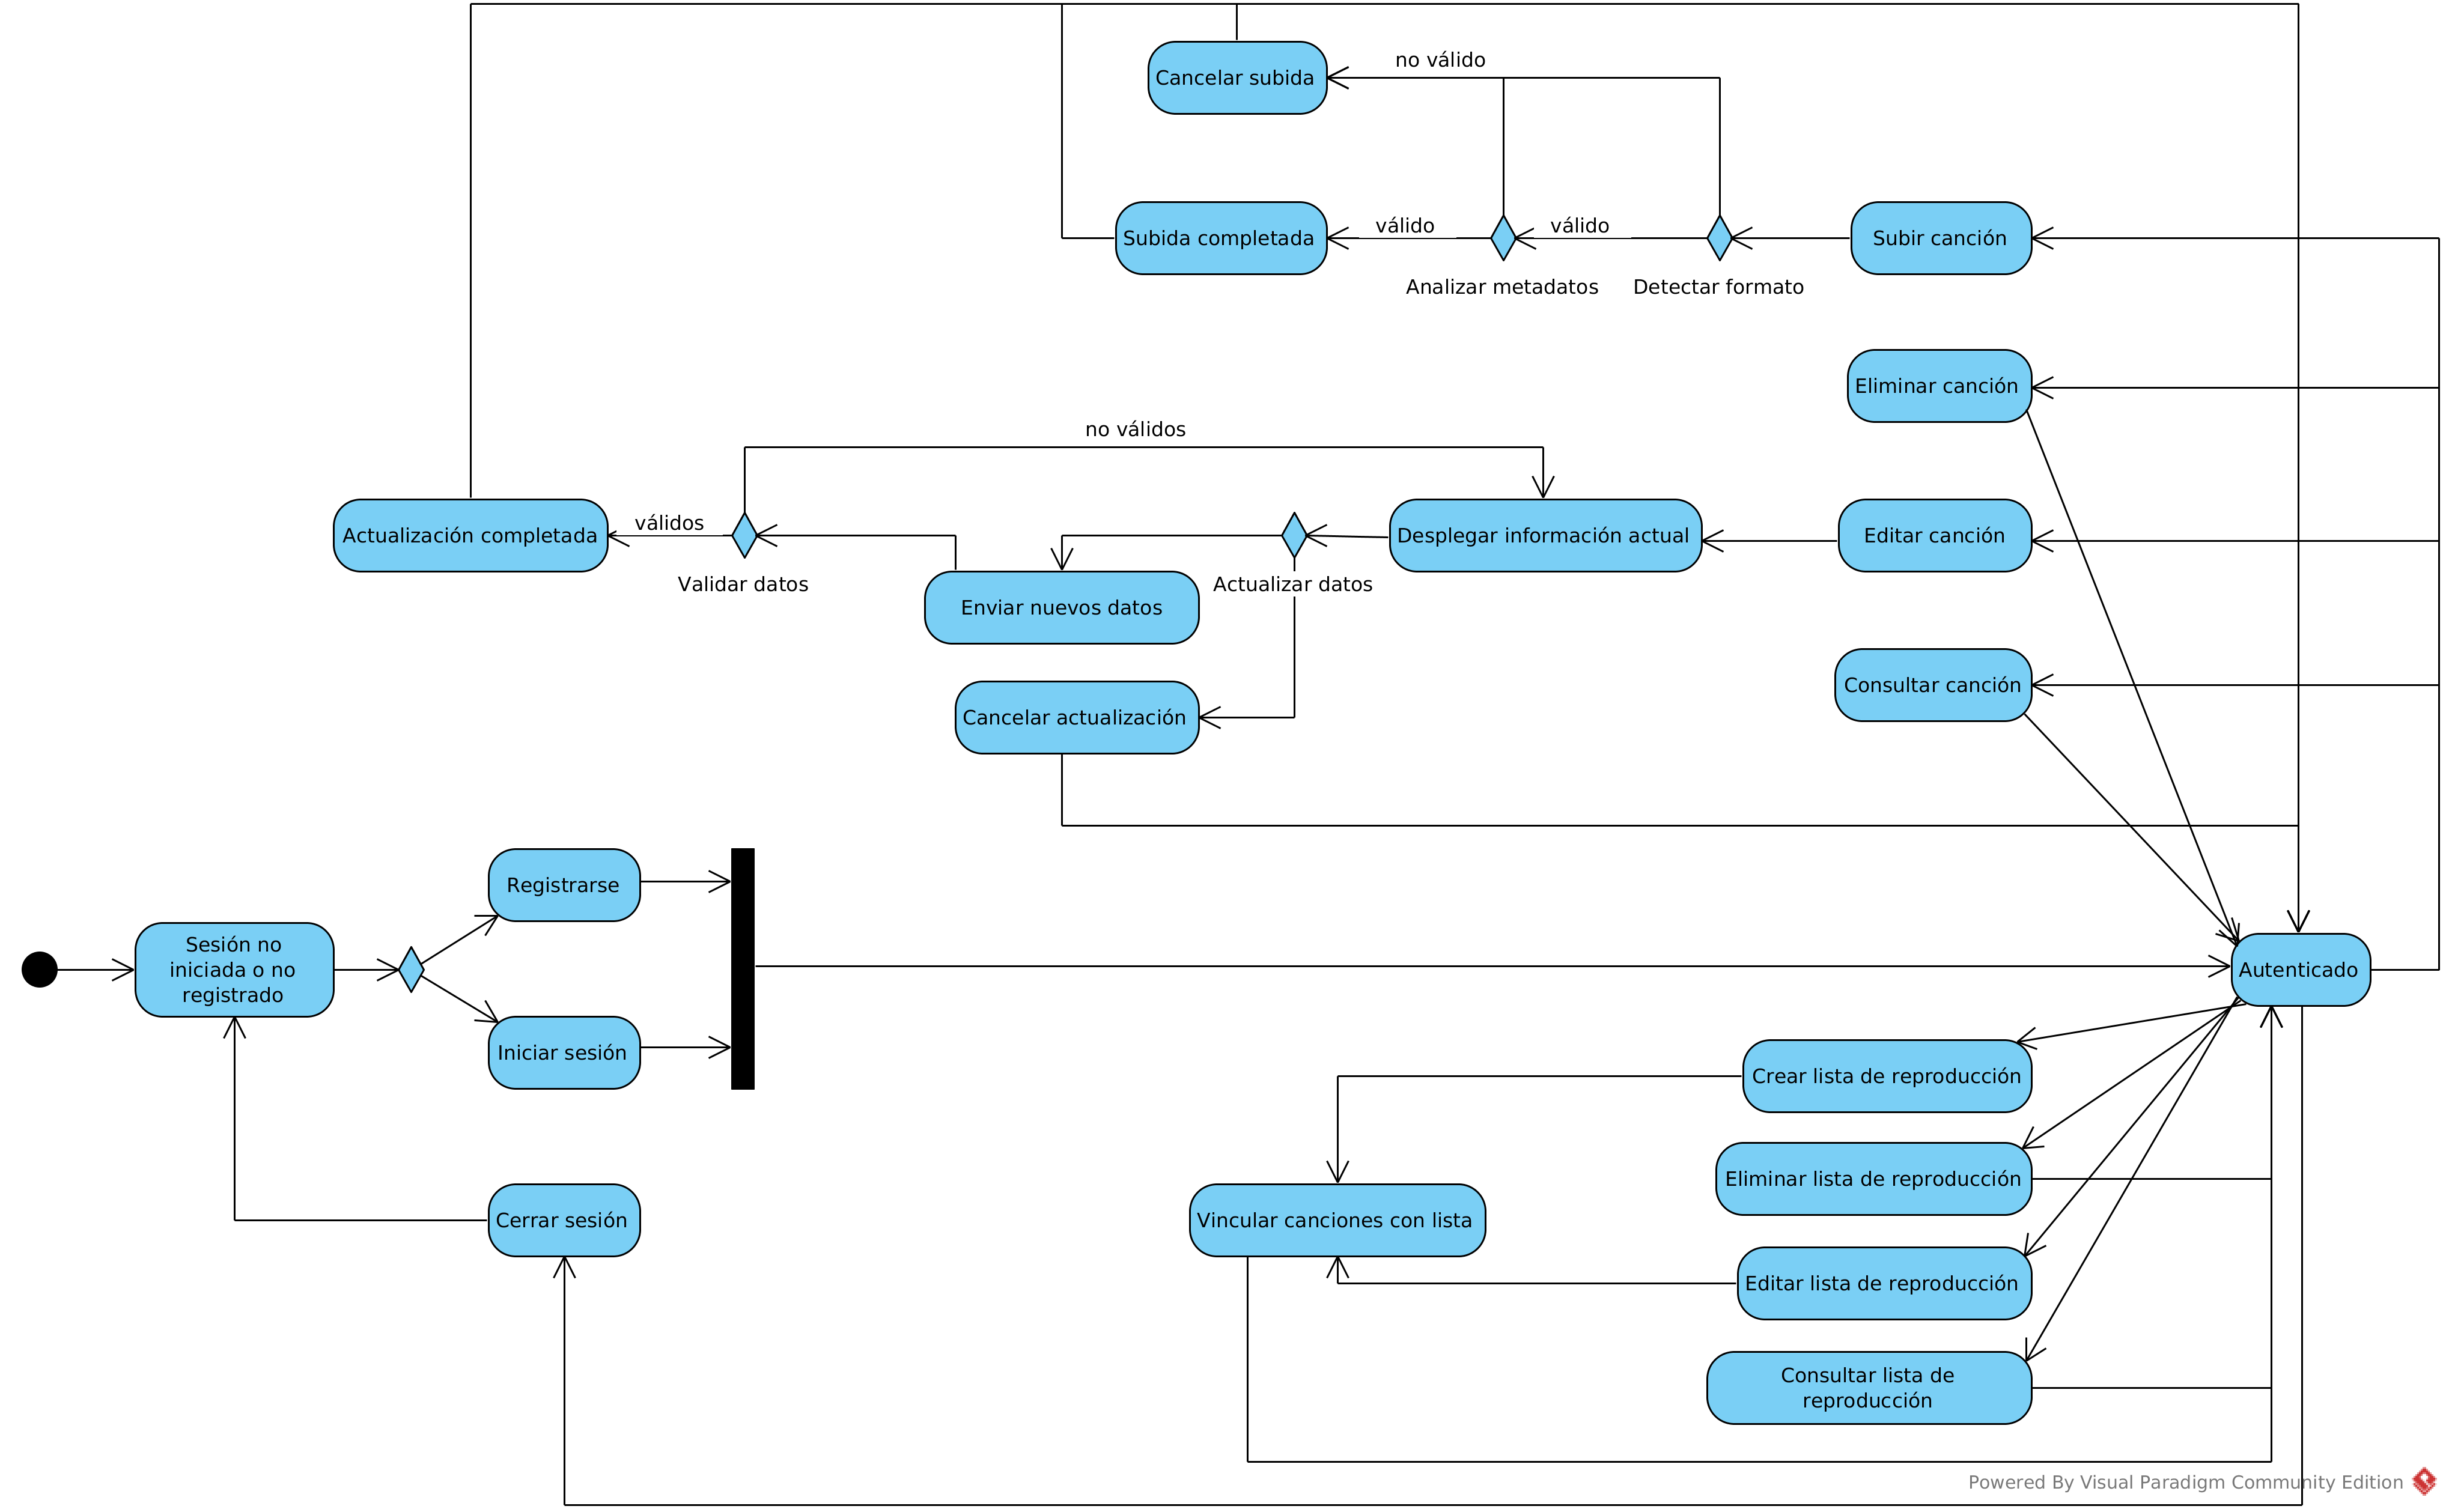
\includegraphics[width=1\textwidth]{../visual_paradigm_uml/Diagrama_actividad_sistema.png}
  \caption{Diagrama de actividad del sistema}
  \label{fig:diag_ac_sis}
  \end{center}
\end{figure}

\subsubsection{Diagrama de clases del diseño}

En el diagrama de clases del diseño se muestra la especificación para las clases software de la aplicación e incluye:

\begin{itemize}
    \item Clases, asociaciones y atributos
    \item Métodos
    \item Navegabilidad
    \item Dependencias
\end{itemize}

A continuación se muestra el diagrama de clases del diseño propuesto:

\begin{figure}[H]
  \begin{center}
  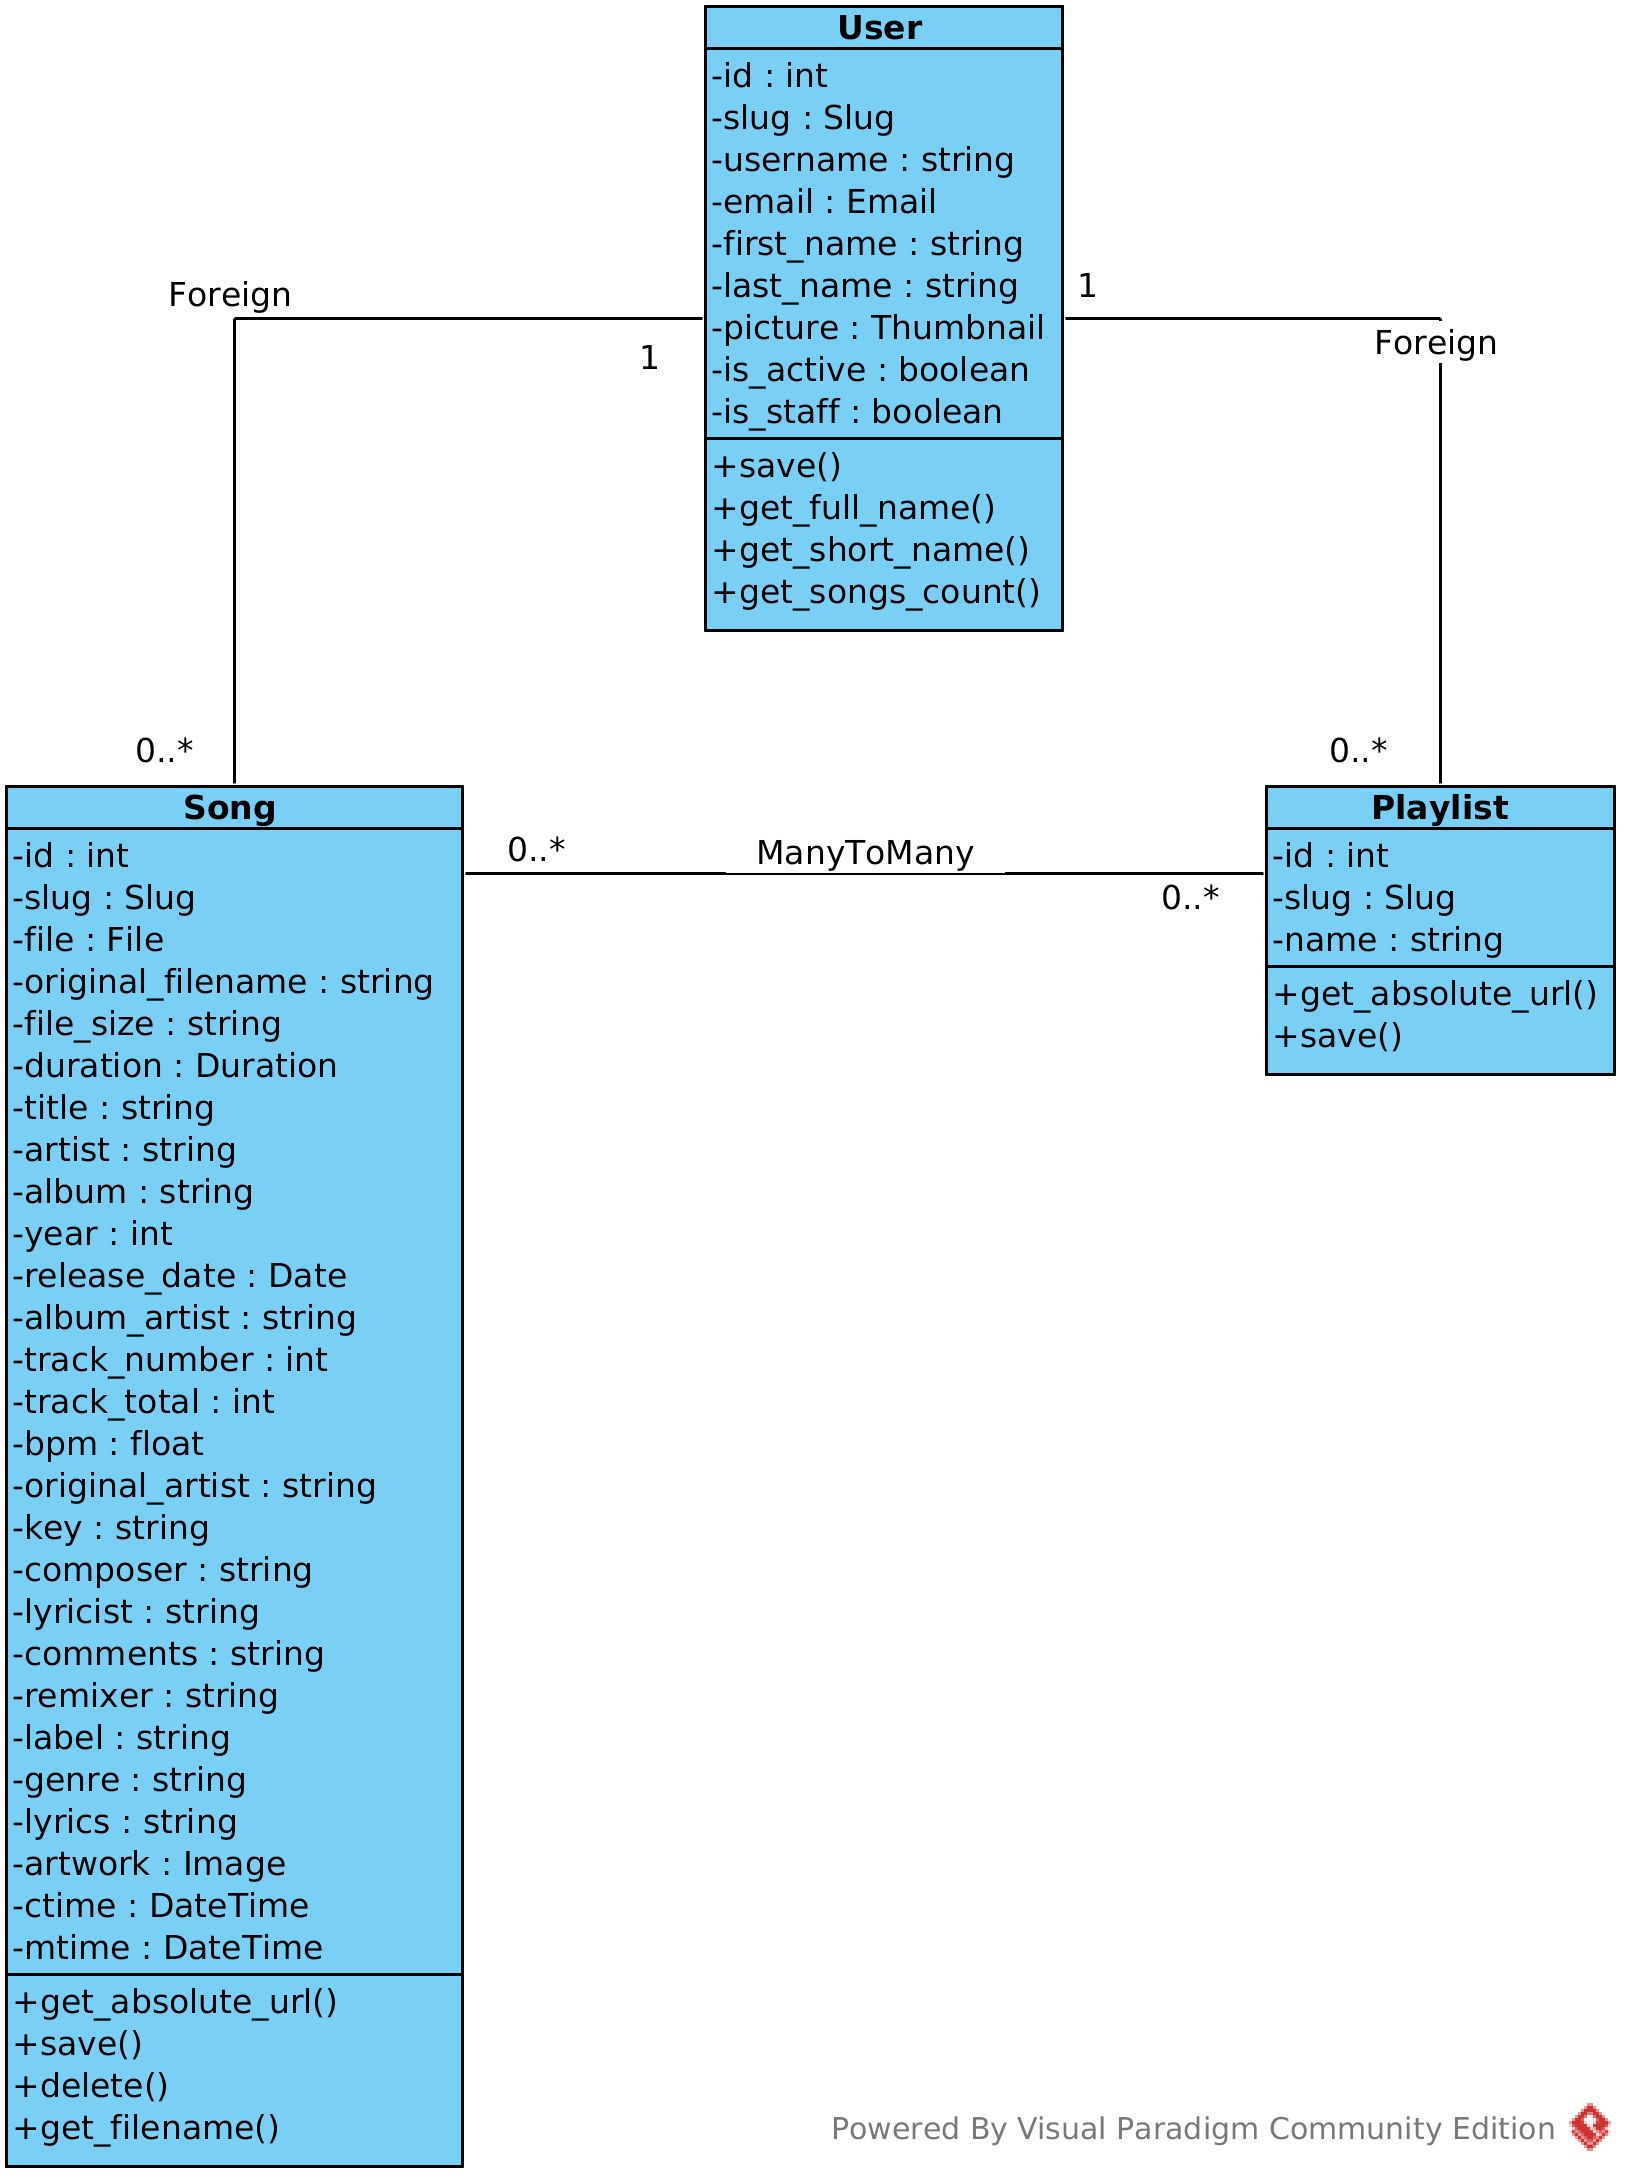
\includegraphics[width=0.8\textwidth]{../visual_paradigm_uml/Diagrama_clases.png}
  \caption{Diagrama de clases del diseño}
  \label{fig:diag_class}
  \end{center}
\end{figure}
